\documentclass[11pt, a4paper]{article} 

\usepackage[utf8]{inputenc}  

\usepackage{caption}    		

\usepackage{etoolbox}    
\usepackage[bottom]{footmisc}  
\usepackage{graphicx}       
\usepackage[hidelinks]{hyperref}		
%\usepackage{listings}
\usepackage{lscape}
\usepackage{euler}     
\usepackage[margin=1in]{geometry}

\usepackage{Sweave}
%\usepackage{C:/Program Files/R/R-3.1.2/share/texmf/tex/latex/Sweave.sty}

\frenchspacing 
%------------------------------------------------------------------------------------------------------
%------------------------------------------------------------------------------------------------------

\begin{document}
\Sconcordance{concordance:sweave_document_TB.tex:sweave_document_TB.Rnw:%
<<<<<<< Updated upstream
1 39 1 1 0 22 1 1 8 4 1 1 7 1 2 9 1 2 2 4 1 1 4 1 1 1 4 20 1}
=======
1 39 1 1 0 24 1 1 7 1 2 6 1 1 4 1 2 3 1}
>>>>>>> Stashed changes



\title{Appendix}

\author{Torfinn and Carolina}

\maketitle

%------------------------------------------------------------------------------------------------------
%------------------------------------------------------------------------------------------------------


\section{Introduction}%------------------------------------------------------------------------------------------------------

We created an appendix of meta-analysis paper. To be able to visualize the output, we used an example dataset taken from Gibson et al. 2011.
The appendix includes forest plots, funnel plots and tables visualizing the results created in the meta-analysis.
\bigskip


%The dataset to be working with should be named ``data.sub''. The conducted analysis using the function rma from the metafor pacakge should be renamed as such: rma of a random effects model should be named ``rma.RE'' and an rma of a fixed effects model should be named ``rma.FE'' in order for the automatisation to work. IF a meta-regression has been conducted, it should be called ``rma.RE.meta'' or ``rma.FE.meta'' respectively. Other than that, the metafor package in R needs to be installed.  






\begin{figure}[htbp]
\captionsetup{width=0.6\textwidth}
\centering
\includegraphics[width=1\textwidth]{sweave_document_TB-forest}
\caption{Forest plot of a random effects model. The study and its respectice effect size (ES) is shown. The weight given to the study (\%) as well as the effect size (ES) [+- 95\% CI] are shown.}
\label{fig:forestplot}
\end{figure}

If the effect sizes in the forest plot vary too  much, then heterogeneity should be explored in more depth. This is done by taking the explanatory variabales into account in a meta-regression. When taking various explanatory variables (moderators) into account, the resulting forest plot shows the   



\begin{figure}[htbp]
\captionsetup{width=0.6\textwidth}
\centering
\includegraphics[width=1\textwidth]{sweave_document_TB-forestreg}
\caption{Forest plot of a random effects regression model. The column on the left represents the study. The weighted percentage is shown as well as the effect size (ES) [+- 95\% CI]}
\label{fig:forestplotreg}
\end{figure}



%Table with values for ES, SE (ES),pES, CI, I2, Egger value and fasil-sage number. An rma with various moderators can be loaded into this table as well. 


\bigskip




% latex table generated in R 3.1.2 by xtable 1.7-4 package
% Tue Nov 25 16:35:10 2014
\begin{table}[ht]
\centering
\caption{Results of the meta-analysis.ES = Effect Size, Q = Test for residual heterogeneity, $I^2$ = residual heterogeneity, Egger's test and the fails-safe number for publication bias testing.} 
{\footnotesize
\scalebox{0.9}{
\begin{tabular}{rccccccccccc}
  \hline
 & {ES} & \parbox{1cm}{SE of ES} & CI (lb) & CI (ub) & P(ES) & Q & P(Q) & I^2 & Egger & P(Egger) & FSN \\ 
  \hline
Meta-Analysis & -0.28 & 0.12 & -0.52 & -0.04 & 0.02 & 47.05 & 0.12 & 27.22 & -0.44 & 0.66 & 77.00 \\ 
   \hline
\end{tabular}
}
}
\end{table}

\bigskip

%Table of the meta-regression. In this case only for one moderator. 


% latex table generated in R 3.1.2 by xtable 1.7-4 package
% Tue Nov 25 16:35:10 2014
\begin{table}[ht]
\centering
\caption{Results of the meta-regression (mixed-effects model). The model results are shown taking a moderator into account and displaying the coefficients. Results for the whole model are displayed as Q = Test for residual heterogeneity, $I^2$ = residual heterogeneity and QM = Test of Moderators.} 
{\footnotesize
\scalebox{0.9}{
\begin{tabular}{rccccc|ccccc}
  \hline
 & {ES} & \parbox{1cm}{SE of ES} & CI (lb) & CI (ub) & P(ES) & Q & P(Q) & I^2 & QM & P(QM) \\ 
  \hline
intrcpt & -0.353 & 0.766 & -1.85 & 1.15 & 0.645 & 22.7 & 0.54 & 0.000493 & 24.4 & 0.0278 \\ 
  continentAS & -0.377 & 0.423 & -1.21 & 0.452 & 0.373 &  &  &  &  &  \\ 
  continentCA & -0.0485 & 0.61 & -1.24 & 1.15 & 0.937 &  &  &  &  &  \\ 
  continentSA & -0.627 & 0.375 & -1.36 & 0.108 & 0.0945 &  &  &  &  &  \\ 
  metricric & 0.119 & 0.254 & -0.38 & 0.617 & 0.641 &  &  &  &  &  \\ 
  disturbanceagf & 0.331 & 0.745 & -1.13 & 1.79 & 0.657 &  &  &  &  &  \\ 
  disturbanceagr & 0.701 & 0.936 & -1.13 & 2.54 & 0.454 &  &  &  &  &  \\ 
  disturbancebur & 0.723 & 0.731 & -0.709 & 2.15 & 0.322 &  &  &  &  &  \\ 
  disturbanceoth & 0.728 & 0.903 & -1.04 &  2.5 & 0.42 &  &  &  &  &  \\ 
  disturbancepas & -0.0589 & 0.979 & -1.98 & 1.86 & 0.952 &  &  &  &  &  \\ 
  disturbancepla & -0.203 & 0.868 & -1.9 &  1.5 & 0.815 &  &  &  &  &  \\ 
  disturbancesec & 0.399 & 0.723 & -1.02 & 1.82 & 0.581 &  &  &  &  &  \\ 
  disturbancesel & 0.796 & 0.691 & -0.559 & 2.15 & 0.25 &  &  &  &  &  \\ 
  disturbanceshd & -0.908 & 0.783 & -2.44 & 0.626 & 0.246 &  &  &  &  &  \\ 
   \hline
\end{tabular}
}
}
\end{table}




%<< echo=FALSE, eval=TRUE >>=
%sens.RE = leave1out(rma.RE)
%if ((length(which(sens.RE$I2 < 25))) > 0) {
%  (which(sens.RE$I2 < 25))
%} else {
%      (which((rma.RE$I2 - sens.RE$I2) > 4))}
%@


% 
% <<xtable2, results = tex, echo=FALSE>>=
% 
% print(xtable(mytable, caption = paste("Results of the meta-analysis.ES = Effect Size, Q = Test for residual heterogeneity, $I^2$ = residual heterogeneity, Egger's test and the fails-safe number for publication bias testing."),align = "rccccccccccc"),caption.placement = "top", size ="footnotesize", scalebox = 0.9, sanitize.text = force)
% @
% 



\begin{figure} [ht]
\captionsetup{width=0.6\textwidth}
\centering
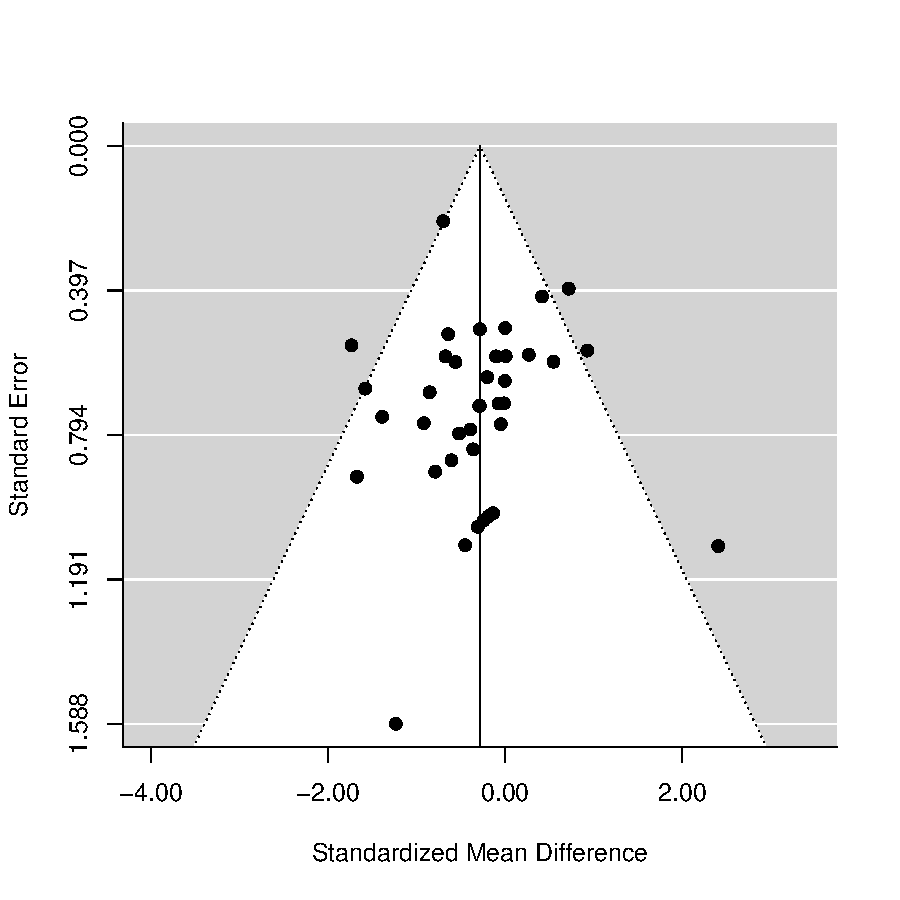
\includegraphics[width=0.7\textwidth]{sweave_document_TB-funnelplot}
\caption{Funnel plot of random effects model displaying possible publication bias. The true ES is displayed by the solid verical line.}
\end{figure}

To assess possible publication bias, funnel plots can be used for visualization purposes.When publication bias is absent, the plot should have a symmetrical shape of a funnel around the mean effect size. This is because the precision of the estimation of effect size, should increase with sample size (smaller standard error). 




\begin{figure} [ht]
\captionsetup{width=0.6\textwidth}
\centering
\includegraphics[width=1\textwidth]{sweave_document_TB-diagnostics}
\caption{Diagnostic plots for diagnostics of meta analysis. Standardized residual plot, normal Q-Q plot, Baujat heterogeneity plot and Galbrath's radial plot are shown.}
\label{fig:diagnostics}
\end{figure}

The Baujat plot detects sources of heterogeneity. Studies which are aggregated to the far left of the plot contribute to more heterogeneity in the analysis. Plots which have hight a high contribution to the overall heterogeneity and have a high influence on the overall result, should be looked at more critically and compare these studies to the results obtained in the sensitivity analysis table REF!!!!!.  


The Galbraith plot provides visual information on the heterogeneity of the meta-analysis. Values which are closer to the origin have a higher SE and are therefore less precise than values aggregated away from the origin. The curved axis indicates the individual observed effect sizes or outcomes and the line coming from (0,0) indicates the individual effect size or outcome for that specific point. 





%<<>>=
%Sweave("sweave_document_TB.Rnw", syntax="SweaveSyntaxNoweb")
%#options(SweaveSyntax="SweaveSyntaxNoweb")
%@
\bigskip

\Sexpr
{
 if (rma.RE$pval < 0.05) {
  if (length(which(sens.RE$pval > 0.05) > 0)) { 
  paste0("The leave-one out analysis shows that the effect size of the meta-analysis 
is not significant anymore when following study(ies) is left out:", which(sens.RE$pval > 0.05)) 
  } else {
    paste0("The leave-one out analysis shows that no left-out studies yield non-significance. This means that the meta-analysis is robust.")}
} else {
  if (length(which(sens.RE$pval < 0.05) > 0)) { 
  paste0("The leave-one out analysis shows that significance is yielded by leaving out the following study(ies):", which(sens.RE$pval < 0.05))  
  } else {
    paste0("The leave-one out analysis shows that no left-out studies yield significance of the original meta analysis.")}
  }
}



\end{document}
